% !TeX root = ../results-review.tex
\section{Experimental results and analysis}
\label{sec:results}

This chapter presents the model evaluation results 
and examines what the recorded SQL trajectories reveal beyond final-result correctness.

\subsection{Collection and coverage}
\label{sec:results-coverage}

Both models completed two runs of the custom Chinook-Bench-200 benchmark.
Each run was collected separately and contained the same 195 benchmark cases,
including the five interactive cases with two turns each.
Across four runs, this produced 780 case evaluations and
800 primary question turns.

\hyperref[tab:results-coverage]{Table~\ref*{tab:results-coverage}} summarises the recorded coverage.
Nova 1, Nova 2, Haiku 1 and Haiku 2 identify each model's two repetitions.
All benchmark cases were present in every run.

\begin{table}[H]
\centering
{\small
\setlength{\tabcolsep}{4pt}
\begin{tabularx}{\textwidth}{@{}>{\raggedright\arraybackslash}Xrrrr@{}}
\toprule
\textbf{Coverage} & \textbf{Nova 1} & \textbf{Nova 2} & \textbf{Haiku 1} & \textbf{Haiku 2} \\
\midrule
Benchmark cases recorded & 195 & 195 & 195 & 195 \\
\addlinespace[0.4em]
Primary question turns & 200 & 200 & 200 & 200 \\
\addlinespace[0.4em]
Saved interactions, including continuations & 216 & 216 & 213 & 213 \\
\addlinespace[0.4em]
Standalone cases scored & 160 & 160 & 160 & 160 \\
\addlinespace[0.4em]
Ambiguity cases assessed for clarification & 20 & 20 & 20 & 20 \\
\addlinespace[0.4em]
Ambiguity cases assessed against reference results & 16 & 16 & 13 & 13 \\
\addlinespace[0.4em]
Interactive turns scored & 10 & 10 & 10 & 10 \\
\addlinespace[0.4em]
Safety cases manually reviewed & 10 & 10 & 10 & 10 \\
\addlinespace[0.4em]
System-error trajectories & 0 & 0 & 0 & 0 \\
\bottomrule
\end{tabularx}
}
\caption{Coverage across the four runs. Rows are not additive (Source: Author, 2026).}
\label{tab:results-coverage}
\end{table}

Saved interactions exceeded the 200 primary turns because the runner provided
additional replies after clarification requests.
Nova Lite received 16 scripted replies per run, giving 216
interactions, while Haiku received 13, giving 213.
Ambiguity cases were assessed for clarification behaviour, 
but their result correctness was scored only for questions that received the scripted reply.

Also, it is worth noting that the remaining four Nova cases and seven Haiku cases 
were excluded from post-clarification accuracy calculations.
This difference followed the evaluation policy described in \hyperref[sec:clarification-interaction-safety-metrics]{Section~\ref*{sec:clarification-interaction-safety-metrics}}.

The primary analysis included all 160 standalone questions per run;
the sensitivity check used 154,
as described in \hyperref[sec:sensitivity-check]{Section~\ref*{sec:sensitivity-check}}.
The exclusions applied only to the sensitivity check and did not change the
coverage or denominators of the primary results.

The completed targeted manual review provided a further check on ten selected
cases, with agreement on their recorded outcomes. Its selection and limits are
described in \hyperref[sec:targeted-manual-trajectory-review]{Section~\ref*{sec:targeted-manual-trajectory-review}}.

\subsection{Final and direct correctness}
\label{sec:results-correctness}

\subsubsection{Final and clean direct success rates}

Final Success Rate (FSR) is the share of standalone questions ending with a
correct result. Clean Direct Success Rate (CDSR) counts those solved with one
correct SQL attempt, no redundant action and no unnecessary clarification.
Both use all 160 standalone questions as their denominator. In Nova's first
run, 122 questions succeeded directly and five after recovery, giving
127 final successes. Thus,
\[
\mathrm{FSR} = 100 \times \frac{127}{160} = 79.38\%, \qquad
\mathrm{CDSR} = 100 \times \frac{122}{160} = 76.25\%.
\]

Haiku achieved more correct final results than Nova in both repetitions
(\hyperref[fig:results-correctness]{Figure~\ref*{fig:results-correctness}}). The difference was 19 questions in the
first repetition and 23 in the second. With 160 questions per run, these
correspond to FSR differences of 11.88 and 14.38 percentage points.
Haiku also had more clean direct successes. Its advantage therefore
remained when considering only cases that succeeded without additional actions.

\begin{figure}[H]
\centering
% Generated by analysis/build-results-review.py from verified run summaries.
\begingroup
\definecolor{finalbar}{HTML}{24557A}
\definecolor{directbar}{HTML}{168475}
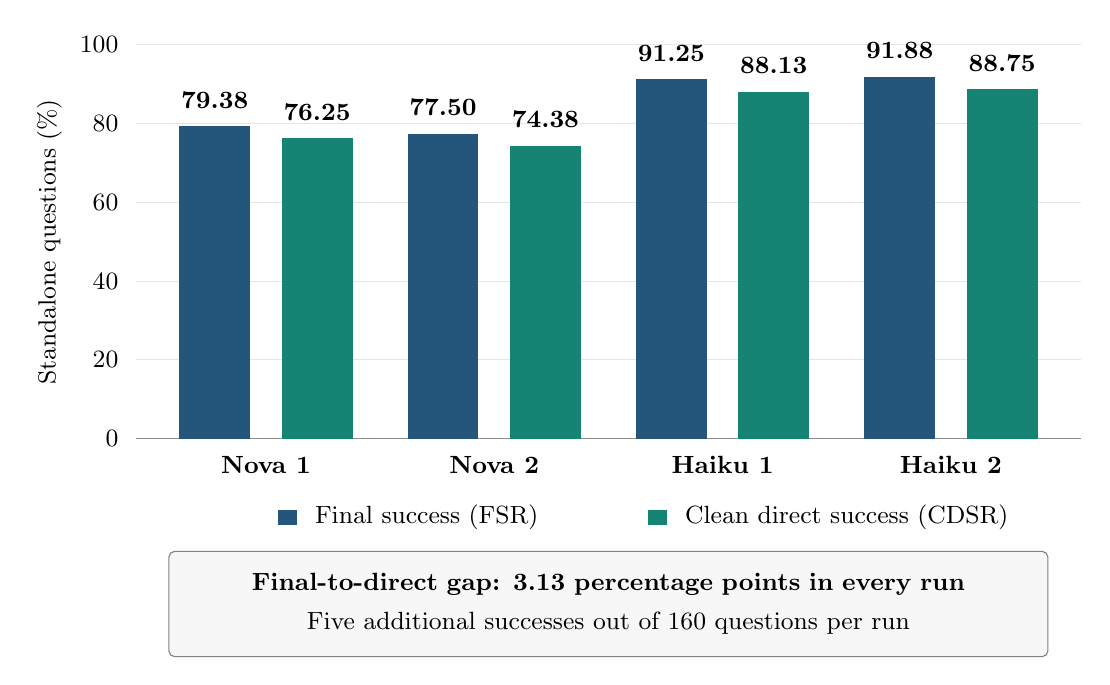
\begin{tikzpicture}[x=1cm,y=0.05cm,font=\small]
\foreach \y in {0,20,40,60,80,100} {
  \draw[black!10] (0,\y) -- (12,\y);
  \node[anchor=east] at (-.1,\y) {\y};
}
\draw[black!45,line width=.6pt] (0,0) -- (12,0);
\node[rotate=90] at (-1.1,50) {Standalone questions (\%)};
\node[below,font=\small\bfseries] at (1.65,-2) {Nova 1};
\fill[finalbar] (0.5499999999999998,0) rectangle (1.45,79.375);
\node[above=3pt,font=\small\bfseries] at (0.9999999999999999,79.375) {79.38};
\fill[directbar] (1.8499999999999999,0) rectangle (2.75,76.25);
\node[above=3pt,font=\small\bfseries] at (2.3,76.25) {76.25};
\node[below,font=\small\bfseries] at (4.55,-2) {Nova 2};
\fill[finalbar] (3.4499999999999997,0) rectangle (4.35,77.5);
\node[above=3pt,font=\small\bfseries] at (3.9,77.5) {77.50};
\fill[directbar] (4.75,0) rectangle (5.65,74.375);
\node[above=3pt,font=\small\bfseries] at (5.2,74.375) {74.38};
\node[below,font=\small\bfseries] at (7.449999999999999,-2) {Haiku 1};
\fill[finalbar] (6.349999999999999,0) rectangle (7.249999999999999,91.25);
\node[above=3pt,font=\small\bfseries] at (6.799999999999999,91.25) {91.25};
\fill[directbar] (7.6499999999999995,0) rectangle (8.549999999999999,88.125);
\node[above=3pt,font=\small\bfseries] at (8.1,88.125) {88.13};
\node[below,font=\small\bfseries] at (10.35,-2) {Haiku 2};
\fill[finalbar] (9.25,0) rectangle (10.149999999999999,91.875);
\node[above=3pt,font=\small\bfseries] at (9.7,91.875) {91.88};
\fill[directbar] (10.55,0) rectangle (11.45,88.75);
\node[above=3pt,font=\small\bfseries] at (11.0,88.75) {88.75};
\fill[finalbar] (1.8,-22) rectangle (2.05,-18);
\node[anchor=west] at (2.15,-20) {Final success (FSR)};
\fill[directbar] (6.5,-22) rectangle (6.75,-18);
\node[anchor=west] at (6.85,-20) {Clean direct success (CDSR)};
\node[draw=black!50,fill=black!3,rounded corners=2pt,
  inner sep=8pt,align=center,text width=10.6cm] at (6,-42)
  {\textbf{Final-to-direct gap: 3.13 percentage points in every run}\\[3pt]
   Five additional successes out of 160 questions per run};
\end{tikzpicture}
\endgroup

\caption{Final Success Rate (FSR) and Clean Direct Success Rate (CDSR), each based on 160 questions per run (Source: Author, 2026).}
\label{fig:results-correctness}
\end{figure}

Between repetitions, final-success and clean-direct counts changed slightly.
Nova's final-success count fell by three and Haiku's increased by one. 
The clean-direct counts changed by the same amounts.

\subsubsection{What the equal gap shows}

Each run had five more final successes than clean direct successes.
With 160 standalone questions per run, the Final-to-Direct Gap (FDG),
the difference between FSR and CDSR, was therefore 3.13 percentage points
in all four runs.
All five cases in each run were execution-error recoveries;
no other type of successful trajectory contributed to the gap.

Despite the equal count, the models recovered on different questions.
For example, CB200-E030 required recovery in both Haiku runs, 
and Nova recovered CB200-M026 in both runs. 
Nova's recovered cases also changed between repetitions.

\subsubsection{Share of successes that were not direct}
RQ1 concerns the proportion of successful cases, so its denominator differs
from the gap: \hyperref[tab:results-nondirect-share]{Table~\ref*{tab:results-nondirect-share}}
reports successes that were not clean direct successes as a share of all final successes.
In these runs, this share equals Recovered Success Contribution (RSC), which
measures how much final success involved recovery. Every non-direct success
was a recovery, so Nova's first-run RSC was 3.94\%:
five recovered successes out of 127 final successes.
Unlike FDG, RSC uses only final successes as its denominator.

\begin{table}[H]
\centering
{\small
\setlength{\tabcolsep}{4pt}
\begin{tabularx}{\textwidth}{@{}>{\raggedright\arraybackslash}Xrrr@{}}
\toprule
\textbf{Run} & \textbf{Recovered successes} & \textbf{Final successes} & \textbf{RSC (\%)} \\
\midrule
Nova 1 & 5 & 127 & 3.94 \\
\addlinespace[0.4em]
Nova 2 & 5 & 124 & 4.03 \\
\addlinespace[0.4em]
Haiku 1 & 5 & 146 & 3.42 \\
\addlinespace[0.4em]
Haiku 2 & 5 & 147 & 3.40 \\
\bottomrule
\end{tabularx}
}
\caption{Recovered Success Contribution (RSC) by model and repetition (Source: Author, 2026).}
\label{tab:results-nondirect-share}
\end{table}

For RQ1, execution-error recovery accounted for 3.40--4.03\% of final successes,
with five recovered cases in every run
(\hyperref[tab:results-nondirect-share]{Table~\ref*{tab:results-nondirect-share}}).
The smaller shares for Haiku reflect its larger number of final successes,
not fewer recovered cases. Final correctness alone did not distinguish these
recoveries from direct successes. These results do not show how many
cases would have failed under a different retry policy, since that condition
was not tested.

\subsection{Recovery and terminal failure}
\label{sec:results-recovery}

\subsubsection{Terminal trajectory classes}

The models differed in their terminal failures, although both recovered on five questions per run.
\hyperref[fig:results-trajectories]{Figure~\ref*{fig:results-trajectories}} shows the recorded
trajectory classes. 
Nova ended with 33 and 36 unsuccessful cases, compared with 14 and 13 for Haiku. 
Nova's 33 first-run failures comprised 27 semantic failures,
five execution failures and one no-SQL case.
All of Haiku's terminal failures were executable
results that did not match the reference contract.

\begin{figure}[H]
\centering
% Generated by analysis/build-results-review.py; counts out of 160.
\begingroup
\definecolor{direct}{HTML}{24557A}
\definecolor{recovery}{HTML}{168475}
\definecolor{semantic}{HTML}{E4B15A}
\definecolor{execution}{HTML}{A34C40}
\definecolor{nosql}{HTML}{555555}
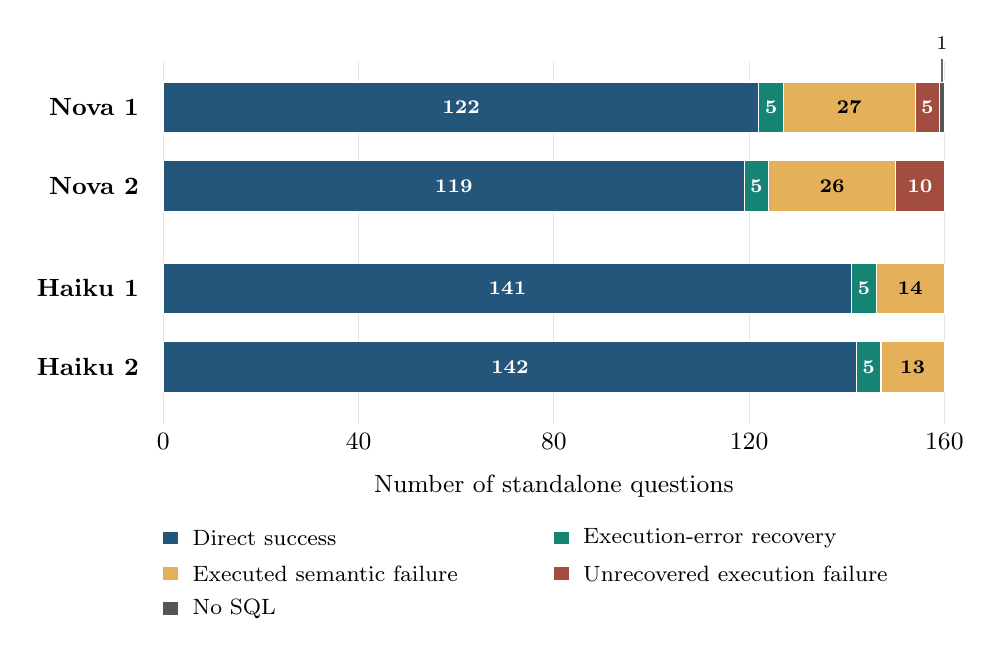
\begin{tikzpicture}[x=0.062cm,y=1cm,font=\small]
\foreach \x in {0,40,80,120,160} {
  \draw[black!10] (\x,-.1) -- (\x,4.5);
  \node[below] at (\x,-.1) {\x};
}
\node at (80,-.9) {Number of standalone questions};
\node[anchor=east,font=\small\bfseries] at (-3,3.92) {Nova 1};
\filldraw[fill=direct,draw=white,line width=.4pt] (0,3.6) rectangle (122,4.24);
\node[text=white,font=\scriptsize\bfseries] at (61.0,3.92) {122};
\filldraw[fill=recovery,draw=white,line width=.4pt] (122,3.6) rectangle (127,4.24);
\node[text=white,font=\scriptsize\bfseries] at (124.5,3.92) {5};
\filldraw[fill=semantic,draw=white,line width=.4pt] (127,3.6) rectangle (154,4.24);
\node[text=black,font=\scriptsize\bfseries] at (140.5,3.92) {27};
\filldraw[fill=execution,draw=white,line width=.4pt] (154,3.6) rectangle (159,4.24);
\node[text=white,font=\scriptsize\bfseries] at (156.5,3.92) {5};
\filldraw[fill=nosql,draw=white,line width=.4pt] (159,3.6) rectangle (160,4.24);
\draw[black!60] (159.5,4.24) -- (159.5,4.53);
\node[above,font=\scriptsize] at (159.5,4.53) {1};
\node[anchor=east,font=\small\bfseries] at (-3,2.92) {Nova 2};
\filldraw[fill=direct,draw=white,line width=.4pt] (0,2.6) rectangle (119,3.24);
\node[text=white,font=\scriptsize\bfseries] at (59.5,2.92) {119};
\filldraw[fill=recovery,draw=white,line width=.4pt] (119,2.6) rectangle (124,3.24);
\node[text=white,font=\scriptsize\bfseries] at (121.5,2.92) {5};
\filldraw[fill=semantic,draw=white,line width=.4pt] (124,2.6) rectangle (150,3.24);
\node[text=black,font=\scriptsize\bfseries] at (137.0,2.92) {26};
\filldraw[fill=execution,draw=white,line width=.4pt] (150,2.6) rectangle (160,3.24);
\node[text=white,font=\scriptsize\bfseries] at (155.0,2.92) {10};
\node[anchor=east,font=\small\bfseries] at (-3,1.62) {Haiku 1};
\filldraw[fill=direct,draw=white,line width=.4pt] (0,1.3) rectangle (141,1.94);
\node[text=white,font=\scriptsize\bfseries] at (70.5,1.62) {141};
\filldraw[fill=recovery,draw=white,line width=.4pt] (141,1.3) rectangle (146,1.94);
\node[text=white,font=\scriptsize\bfseries] at (143.5,1.62) {5};
\filldraw[fill=semantic,draw=white,line width=.4pt] (146,1.3) rectangle (160,1.94);
\node[text=black,font=\scriptsize\bfseries] at (153.0,1.62) {14};
\node[anchor=east,font=\small\bfseries] at (-3,0.62) {Haiku 2};
\filldraw[fill=direct,draw=white,line width=.4pt] (0,0.3) rectangle (142,0.94);
\node[text=white,font=\scriptsize\bfseries] at (71.0,0.62) {142};
\filldraw[fill=recovery,draw=white,line width=.4pt] (142,0.3) rectangle (147,0.94);
\node[text=white,font=\scriptsize\bfseries] at (144.5,0.62) {5};
\filldraw[fill=semantic,draw=white,line width=.4pt] (147,0.3) rectangle (160,0.94);
\node[text=black,font=\scriptsize\bfseries] at (153.5,0.62) {13};
\fill[direct] (0,-1.6300000000000001) rectangle (3,-1.47);
\node[anchor=west,font=\footnotesize] at (4,-1.55) {Direct success};
\fill[recovery] (80,-1.6300000000000001) rectangle (83,-1.47);
\node[anchor=west,font=\footnotesize] at (84,-1.55) {Execution-error recovery};
\fill[semantic] (0,-2.08) rectangle (3,-1.92);
\node[anchor=west,font=\footnotesize] at (4,-2.0) {Executed semantic failure};
\fill[execution] (80,-2.08) rectangle (83,-1.92);
\node[anchor=west,font=\footnotesize] at (84,-2.0) {Unrecovered execution failure};
\fill[nosql] (0,-2.5300000000000002) rectangle (3,-2.37);
\node[anchor=west,font=\footnotesize] at (4,-2.45) {No SQL};
\end{tikzpicture}
\endgroup

\caption{Standalone trajectory classes. Segment labels give counts out of 160 questions per run (Source: Author, 2026).}
\label{fig:results-trajectories}
\end{figure}

Semantic failures were the largest group of terminal failures in every run.
This distribution is presented in \hyperref[fig:results-trajectories]{Figure~\ref*{fig:results-trajectories}} 
with Nova having 27 and 26 and Haiku 14 and 13 such cases.
These counts should not all be read as evidence of faulty analytical reasoning.
The sensitivity analysis mentioned earlier examines cases affected by output conventions and
reference assumptions.

\subsubsection{From the first attempt to the final outcome}
Nova encountered execution errors on 14 and 20 questions in its first and second runs respectively, 
while Haiku had only five in each run.
Each question was counted once and the number of attempts it contained did not matter. 
Both Nova and Haiku recovered on five of these questions in each run.

The remaining nine cases in Nova's first run ended with either an executable but incorrect result
(four cases) or an execution error (five cases). 
In its second run, five ended with incorrect results and ten with execution errors 
(see \hyperref[tab:first-terminal-outcomes]{Table~\ref*{tab:first-terminal-outcomes}}). 
These results show that successful execution was not enough to count as a recovery.
The query result also had to match the reference answer.

These cases also show what a final failure label leaves out.
Some of Nova's semantic failures followed an execution error and others were
incorrect on the first attempt. 
They ended in the same category, but reached it through different paths.
The first-to-final comparison identifies that difference, 
but explaining the SQL changes requires the intermediate attempts.

\begin{table}[H]
\centering
{\small
\setlength{\tabcolsep}{4pt}
\begin{tabularx}{\textwidth}{@{}>{\raggedright\arraybackslash}X>{\raggedright\arraybackslash}Xrrrr@{}}
\toprule
\textbf{First outcome} & \textbf{Terminal outcome} & \textbf{Nova 1} & \textbf{Nova 2} & \textbf{Haiku 1} & \textbf{Haiku 2} \\
\midrule
Correct & Correct & 122 & 119 & 141 & 142 \\
\addlinespace[0.4em]
Execution error & Correct & 5 & 5 & 5 & 5 \\
\addlinespace[0.4em]
Execution error & Semantic error & 4 & 5 & 0 & 0 \\
\addlinespace[0.4em]
Execution error & Execution error & 5 & 10 & 0 & 0 \\
\addlinespace[0.4em]
Semantic error & Semantic error & 23 & 21 & 14 & 13 \\
\addlinespace[0.4em]
No SQL & No SQL & 1 & 0 & 0 & 0 \\
\bottomrule
\end{tabularx}
}
\caption{First and terminal outcomes for standalone questions; each run totals 160 cases (Source: Author, 2026).}
\label{tab:first-terminal-outcomes}
\end{table}

CB200-H043 from Nova's second run illustrates an execution error followed by
an incorrect result. The question asked: ``Show monthly invoice revenue and
cumulative revenue over time.''
\hyperref[lst:executable-mismatch]{Listing~\ref*{lst:executable-mismatch}}
shows the relevant SQL expressions, database feedback and saved results.
The expressions appeared in the selection, grouping and ordering of months;
the rest of the queries is omitted for readability.

\noindent\begin{minipage}{\linewidth}
\begin{lstlisting}[
  basicstyle=\footnotesize\ttfamily,
  backgroundcolor=\color{black!3},
  frame=single,
  rulecolor=\color{black!25},
  framesep=6pt,
  xleftmargin=7pt,
  xrightmargin=7pt,
  caption={Abbreviated two-attempt trajectory and saved results for CB200-H043, Nova repetition 2 (Source: Author, 2026).},
  label={lst:executable-mismatch},
  captionpos=b
]
Attempt 1: execution error
  Month expression: strftime(invoice_date, '%Y-%m')
  Athena: FUNCTION_NOT_FOUND:
          Function 'strftime' not registered

Attempt 2: executed successfully
  Month expression: date_format(invoice_date, 'yyyy-MM')
  Candidate result (only row):
    month    | monthly_revenue | cumulative_revenue
    yyyy-MM  | 2328.6          | 2328.6

Reference result (first of 60 rows):
  invoice_month           | revenue | cumulative_revenue
  2009-01-01 00:00:00.000  | 35.64   | 35.64

Evaluator: Row count differs: expected 60, received 1.
Trajectory class: EXECUTED_SEMANTIC_FAILURE
\end{lstlisting}
\end{minipage}

The retry replaced the unavailable function,
but its saved result contained the literal text \texttt{yyyy-MM} as the month and a single revenue total.
So it did not provide the monthly breakdown the question requested.

As \hyperref[lst:executable-mismatch]{Listing~\ref*{lst:executable-mismatch}}
shows, Athena's successful execution status and the evaluator's correctness
judgment described different things. 
The saved result contained one row instead of the expected 60, so the
trajectory ended in semantic failure despite the retry executing successfully.

There was also one case (CB200-H025) in Nova's first run that did not produce a SQL attempt.
The question asked about the longest interval between each customer's consecutive invoices and
the case was categorised as a no-SQL outcome.
Because of that, it could not contribute to a
comparison of first and last SQL results or to recovery from an initial error.

\subsubsection{Recovery among initially unsuccessful cases}
\label{sec:results-initial-recovery}
Recovery Rate (RR) measures recovery among questions whose first SQL attempt
had an execution error or returned an incorrect result.
In Nova's first run, 37 questions were initially unsuccessful:
14 execution errors and 23 semantic errors. Five eventually returned a
correct result, giving an RR of 13.51\%.
\hyperref[fig:recovery-rates]{Figure~\ref*{fig:recovery-rates}} presents the
RR values and their underlying counts for all four runs.
Haiku's higher RR reflects fewer initially unsuccessful cases,
not more recoveries.

\begin{figure}[H]
\centering
% Generated by analysis/build-results-review.py from verified summaries.
\begingroup
\definecolor{novabar}{HTML}{24557A}
\definecolor{haikubar}{HTML}{168475}
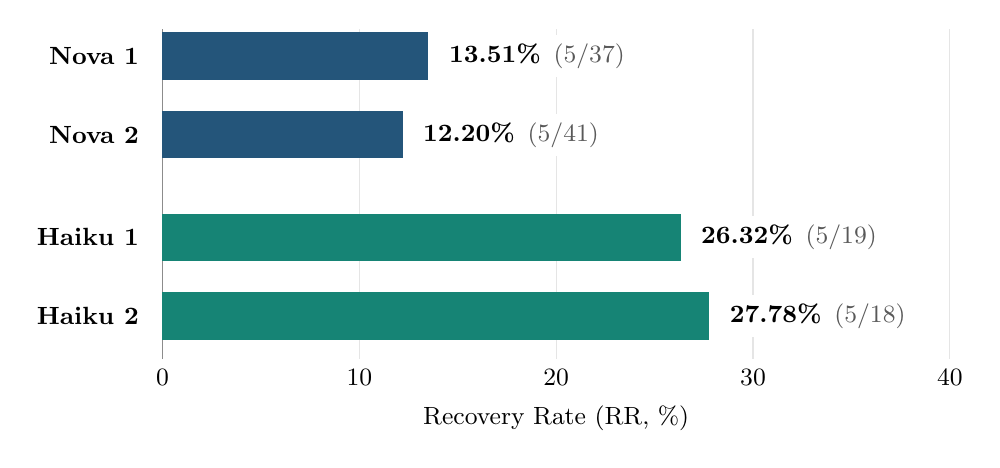
\begin{tikzpicture}[x=.25cm,y=1cm,font=\small]
\foreach \x in {0,10,20,30,40} {
  \draw[black!10] (\x,-.25) -- (\x,3.95);
  \node[below] at (\x,-.25) {\x};
}
\draw[black!45,line width=.6pt] (0,-.25) -- (0,3.95);
\node at (20,-1) {Recovery Rate (RR, \%)};
\node[anchor=east,font=\small\bfseries] at (-.7,3.5999999999999996) {Nova 1};
\fill[novabar] (0,3.3) rectangle (13.51351351351351351351351351,3.9);
\node[anchor=west,fill=white,inner sep=3pt] at (14.11351351351351351351351351,3.5999999999999996) {\textbf{13.51\%}\enspace\textcolor{black!65}{(5/37)}};
\node[anchor=east,font=\small\bfseries] at (-.7,2.5999999999999996) {Nova 2};
\fill[novabar] (0,2.3) rectangle (12.19512195121951219512195122,2.9);
\node[anchor=west,fill=white,inner sep=3pt] at (12.79512195121951219512195122,2.5999999999999996) {\textbf{12.20\%}\enspace\textcolor{black!65}{(5/41)}};
\node[anchor=east,font=\small\bfseries] at (-.7,1.3) {Haiku 1};
\fill[haikubar] (0,1) rectangle (26.31578947368421052631578947,1.6);
\node[anchor=west,fill=white,inner sep=3pt] at (26.91578947368421052631578947,1.3) {\textbf{26.32\%}\enspace\textcolor{black!65}{(5/19)}};
\node[anchor=east,font=\small\bfseries] at (-.7,0.3) {Haiku 2};
\fill[haikubar] (0,0) rectangle (27.77777777777777777777777778,0.6);
\node[anchor=west,fill=white,inner sep=3pt] at (28.37777777777777777777777778,0.3) {\textbf{27.78\%}\enspace\textcolor{black!65}{(5/18)}};
\end{tikzpicture}
\endgroup

\caption{Recovery Rate (RR) by model and repetition. 
Labels show percentages and counts of recovered/initially unsuccessful cases (Source: Author, 2026).}
\label{fig:recovery-rates}
\end{figure}

Question CB200-M026 is a good example of a recovered outcome. 
It asked how many distinct customers were billed in each country. 
In Nova's first run, the first query joined invoices and customers, 
then used \texttt{COUNT(DISTINCT customer\_id)} without qualifying the column.
Athena reported that \texttt{customer\_id} was ambiguous. 
\hyperref[lst:successful-recovery]{Listing~\ref*{lst:successful-recovery}}
shows the first query, the saved error and the corrected expression.
The rest of the second query was unchanged and is omitted.

\noindent\begin{minipage}{\linewidth}
\begin{lstlisting}[
  basicstyle=\footnotesize\ttfamily,
  backgroundcolor=\color{black!3},
  frame=single,
  rulecolor=\color{black!25},
  framesep=6pt,
  xleftmargin=7pt,
  xrightmargin=7pt,
  caption={Execution-error recovery for CB200-M026, Nova repetition 1 (Source: Author, 2026).},
  label={lst:successful-recovery},
  captionpos=b
]
Attempt 1: execution error
  SELECT billing_country,
         COUNT(DISTINCT customer_id) AS distinct_customer_count
  FROM invoices JOIN customers
    ON invoices.customer_id = customers.customer_id
  GROUP BY billing_country

Saved error (position refers to the original one-line SQL):
  Athena query failed: AMBIGUOUS_NAME: line 1:40:
  Column 'customer_id' is ambiguous

Attempt 2: executed successfully
  Corrected expression:
    COUNT(DISTINCT invoices.customer_id)
      AS distinct_customer_count

Evaluator: outcome = correct; resultCorrect = true
Trajectory class: EXECUTION_ERROR_RECOVERED
\end{lstlisting}
\end{minipage}

The following query used \texttt{invoices.customer\_id}, 
executed successfully and matched the reference result. 
Haiku's first-run query, by contrast, used the invoices table alone and
succeeded on its first attempt. 
Both received a correct final outcome,
but only Nova's trajectory included recovery.

\subsubsection{No observed semantic-revision successes}
Every case whose first SQL attempt returned an executable but incorrect
result also ended with a semantic error
(\hyperref[tab:first-terminal-outcomes]{Table~\ref*{tab:first-terminal-outcomes}}).
For RQ2, all observed recoveries therefore followed execution errors.

The instructions encouraged retries after execution errors and answering
after successful execution. This gave the agent a clear signal to correct
failed SQL, but no equivalent signal when an executable result disagreed
with the reference. As described in
\hyperref[sec:runner-evidence]{Section~\ref*{sec:runner-evidence}},
reference comparisons took place offline and were not returned to the agent.

This did not make semantic revision impossible. The agent could still
have issued another query after inspecting its SQL or returned data,
and the evaluator could identify an incorrect first result followed by
a correct final result. However, the experiment did not specifically
prompt semantic revision or test it using correctness feedback.
The zero count therefore does not show that the models were unable
to correct such errors.

\subsection{Responses to database errors}
\label{sec:results-error-responses}

RQ3 asks what happened after an execution-error observation. 
Nova had more failed attempts than Haiku and its errors were often followed by another failed attempt.
Also, Haiku's observed errors were followed by successful execution. 
Additionally, one question could contribute several error
observations, so counts below must be distinguished from the number of
questions that encountered an error.

\subsubsection{Recovery after an execution error}
Observation-conditioned Recovery Rate measures how often questions containing
an execution error ended correctly. Nova's first run had
14 such questions, of which five recovered, giving a rate of 35.71\%.
In its second run, the corresponding rate was 25\% and
100\% in each Haiku run. 
This differs from Recovery Rate (RR)
(see \hyperref[sec:results-initial-recovery]{Section~\ref*{sec:results-initial-recovery}}).
Nova's RR denominator in its first run was 37, including 23 semantic errors
and 14 execution errors. 
Here, only the 14 questions with execution errors are included. 

Haiku had only five questions with an execution error and it was able to recover all of them.
The models also did not face an identical set of failed queries or errors.

\subsubsection{What followed each error observation}
\hyperref[tab:results-error-responses]{Table~\ref*{tab:results-error-responses}}
counts the response to each error observation, using the rules in
\hyperref[sec:error-responses]{Section~\ref*{sec:error-responses}}.
It differentiates successful execution from result correctness.

\begin{table}[H]
\centering
{\small
\setlength{\tabcolsep}{6pt}
\renewcommand{\arraystretch}{1.2}
\begin{tabularx}{\textwidth}{@{}>{\raggedright\arraybackslash}X*{4}{>{\centering\arraybackslash}p{0.115\textwidth}}@{}}
\toprule
\textbf{Response to an error} & \textbf{Nova 1} & \textbf{Nova 2} & \textbf{Haiku 1} & \textbf{Haiku 2} \\
\midrule
\textbf{Retry executed successfully} & \textbf{9} & \textbf{10} & \textbf{5} & \textbf{5} \\
\quad Returned a correct result & 5 & 5 & 5 & 5 \\
\quad Returned an incorrect result & 4 & 5 & 0 & 0 \\
\midrule
\textbf{Retry repeated the same error} & \textbf{71} & \textbf{158} & \textbf{0} & \textbf{0} \\
\quad SQL text unchanged & 36 & 104 & 0 & 0 \\
\quad SQL text changed & 35 & 54 & 0 & 0 \\
\midrule
Retry produced a different error & 3 & 4 & 0 & 0 \\
\addlinespace[0.4em]
No retry & 5 & 10 & 0 & 0 \\
\midrule
\textbf{Total error observations} & \textbf{88} & \textbf{182} & \textbf{5} & \textbf{5} \\
\bottomrule
\end{tabularx}
}
\caption{Responses to standalone execution-error observations. Indented rows break down the preceding total (Source: Author, 2026).}
\label{tab:results-error-responses}
\end{table}

The breakdown above shows that Nova's first run contained 88 error observations.
Of these, 71 were followed by a retry with the same normalised error signature,
giving 80.68\%. 
The second-run proportion was 86.81\%.
Moreover, only five of Nova's executed retries in each run returned correct results; 
the others still failed the reference comparison. 
Haiku's five executed retries per run all returned correct results.

\hyperref[tab:results-error-responses]{Table~\ref*{tab:results-error-responses}} 
also shows that repeated errors followed both unchanged and
changed SQL. Nova sometimes submitted the same query again, but changing
the query did not always resolve the preceding error.

\subsubsection{Error categories and a repeated failure}

Missing-column errors accounted for $85.23\%$ (75/88) of observations
in Nova's first run and $70.33\%$ (128/182) in its second run.
It also recorded 29 type mismatches and 18 \texttt{EXPRESSION\_NOT\_AGGREGATE} errors.
Both Haiku runs contained similar issues but on a smaller scale.
Each contained two missing-column errors, two type mismatches and one unavailable-function error. 

Question CB200-H038 illustrates why that distinction matters. 
In Nova's first run, it produced 32 SQL attempts, all of which failed to execute.
The first failed because \texttt{strftime} function was unavailable. The next
31 reported that the column \texttt{month} could not be resolved.
The first transition was illustrated in
\hyperref[lst:error-transition-example]{Listing~\ref*{lst:error-transition-example}}
in \hyperref[sec:error-responses]{Section~\ref*{sec:error-responses}};
\hyperref[lst:repeated-error-sequence]{Listing~\ref*{lst:repeated-error-sequence}}
below summarises the complete sequence.

\noindent\begin{minipage}{\linewidth}
\begin{lstlisting}[
  basicstyle=\footnotesize\ttfamily,
  backgroundcolor=\color{black!3},
  frame=single,
  rulecolor=\color{black!25},
  framesep=6pt,
  xleftmargin=7pt,
  xrightmargin=7pt,
  caption={Error sequence for CB200-H038, Nova repetition 1 (Source: Author, 2026).},
  label={lst:repeated-error-sequence},
  captionpos=b
]
Attempt 1:     FUNCTION_NOT_FOUND:strftime
Attempts 2-32: COLUMN_NOT_FOUND:month

Responses to the 32 error observations:
  Different error on the next attempt:  1
  Same error on the next attempt:      30
  No further attempt:                  1

Trajectory class: UNRECOVERED_EXECUTION_FAILURE
\end{lstlisting}
\end{minipage}

This single question was responsible for 30 of the 71 repeated-error responses ($42.25\%$)
in Nova's first run. 
It counts as one failure, but its trace shows that it accounted for
many of the run's repeated errors.

\subsubsection{Attempts and the retry policy}
Most questions required only one SQL attempt, but a small group of Nova's
questions produced much longer sequences with multiple attempts.
\hyperref[tab:results-attempt-distribution]{Table~\ref*{tab:results-attempt-distribution}}
shows this distribution. The median was one attempt in every run. 
Nova's maximum was 32 attempts
in its first run and 29 in its second, 
compared with two in each Haiku run.

\begin{table}[H]
\centering
{\small
\setlength{\tabcolsep}{4pt}
\begin{tabularx}{\textwidth}{@{}>{\raggedright\arraybackslash}Xrrrr@{}}
\toprule
\textbf{SQL attempts per question} & \textbf{Nova 1} & \textbf{Nova 2} & \textbf{Haiku 1} & \textbf{Haiku 2} \\
\midrule
None & 1 & 0 & 0 & 0 \\
\addlinespace[0.4em]
One & 145 & 139 & 155 & 155 \\
\addlinespace[0.4em]
Two & 8 & 9 & 5 & 5 \\
\addlinespace[0.4em]
More than two & 6 & 12 & 0 & 0 \\
\midrule
Total questions & 160 & 160 & 160 & 160 \\
Maximum attempts on one question & 32 & 29 & 2 & 2 \\
\bottomrule
\end{tabularx}
}
\caption{SQL-attempt distribution across standalone questions (Source: Author, 2026).}
\label{tab:results-attempt-distribution}
\end{table}

\hyperref[fig:results-attempts]{Figure~\ref*{fig:results-attempts}} shows the
total number of SQL attempts per run. 
Haiku used 165 attempts in each run:
155 questions had one attempt and five had two.
In Nova's first run, six questions had more than two SQL attempts.
These used 4, 5, 5, 12, 23 and 32 attempts, accounting for 81 of the run's 242 attempts. 
In the second run, 12 questions had more than two attempts.
Together, they accounted for 177 of the run's 334 attempts, 
while the remaining 148 questions used 157 attempts.
\hyperref[app:extended-sql-trajectories]{Appendix~\ref*{app:extended-sql-trajectories}}
lists these questions and their attempt counts in each run.

\begin{figure}[H]
\centering
% Generated by analysis/build-results-review.py from saved evaluations.
\begingroup
\definecolor{novabar}{HTML}{24557A}
\definecolor{haikubar}{HTML}{168475}
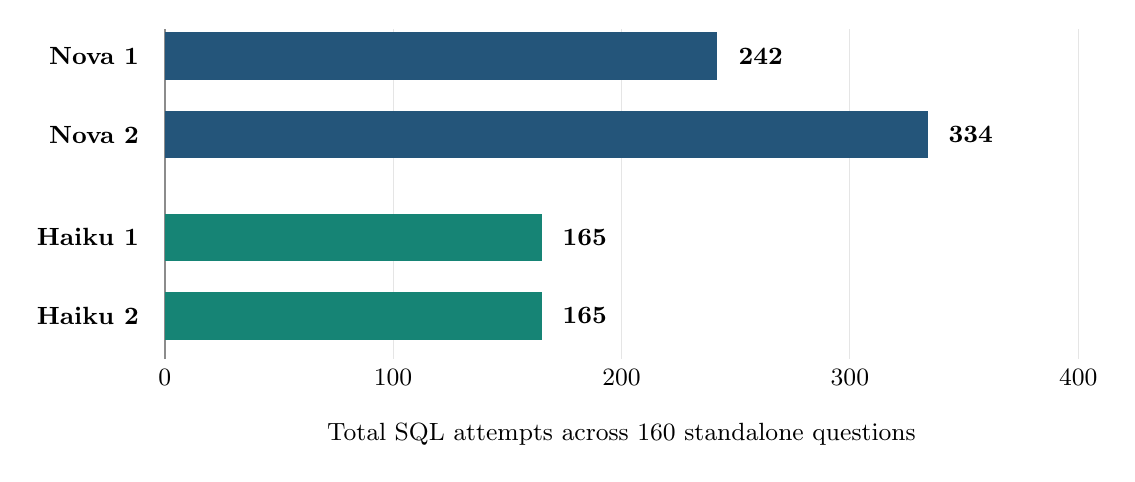
\begin{tikzpicture}[x=.029cm,y=1cm,font=\small]
\foreach \x in {0,100,200,300,400} {
  \draw[black!10] (\x,-.25) -- (\x,3.95);
  \node[below] at (\x,-.25) {\x};
}
\draw[black!45,line width=.6pt] (0,-.25) -- (0,3.95);
\node at (200,-1.2) {Total SQL attempts across 160 standalone questions};
\node[anchor=east,font=\small\bfseries] at (-7,3.6) {Nova 1};
\fill[novabar] (0,3.3000000000000003) rectangle (242,3.9);
\node[anchor=west,font=\small\bfseries] at (247,3.6) {242};
\node[anchor=east,font=\small\bfseries] at (-7,2.6) {Nova 2};
\fill[novabar] (0,2.3000000000000003) rectangle (334,2.9);
\node[anchor=west,font=\small\bfseries] at (339,2.6) {334};
\node[anchor=east,font=\small\bfseries] at (-7,1.3) {Haiku 1};
\fill[haikubar] (0,1.0) rectangle (165,1.6);
\node[anchor=west,font=\small\bfseries] at (170,1.3) {165};
\node[anchor=east,font=\small\bfseries] at (-7,0.3) {Haiku 2};
\fill[haikubar] (0,0.0) rectangle (165,0.6);
\node[anchor=west,font=\small\bfseries] at (170,0.3) {165};
\end{tikzpicture}
\endgroup

\caption{Total SQL attempts by model and repetition (Source: Author, 2026).}
\label{fig:results-attempts}
\end{figure}

Six Nova questions in the first run and 12 in the second exceeded the retry policy of two attempts.
Haiku did not break the policy and had only five questions with two attempts in each run.
The prompt policy was not a hard execution cap, as explained in
\hyperref[sec:protocol]{Section~\ref*{sec:protocol}}.

Contrary to expectations, longer sequences did not always end in failure.
Nova recovered CB200-M039 after five attempts in run 1 and CB200-H007 after three in run 2.
In H007, the first two queries tried to join customers directly to
\texttt{invoice\_items} using its nonexistent \texttt{customer\_id} column.
The third query joined through \texttt{invoices} and returned a correct result.
\hyperref[lst:unchanged-retry-recovery]{Listing~\ref*{lst:unchanged-retry-recovery}}
shows the relevant joins and the saved error. The rest of the SQL is omitted for brevity
and the error position refers to the original one-line query.

\noindent\begin{minipage}{\linewidth}
\begin{lstlisting}[
  basicstyle=\footnotesize\ttfamily,
  backgroundcolor=\color{black!3},
  frame=single,
  rulecolor=\color{black!25},
  framesep=6pt,
  xleftmargin=7pt,
  xrightmargin=7pt,
  caption={Unchanged retry followed by recovery, CB200-H007, Nova repetition 2 (Source: Author, 2026).},
  label={lst:unchanged-retry-recovery},
  captionpos=b
]
Attempts 1 and 2: identical SQL, both failed
  Join excerpt:
    FROM customers c
    JOIN invoice_items ii ON c.customer_id = ii.customer_id

  Saved error on both attempts:
    Athena query failed: COLUMN_NOT_FOUND: line 1:146:
    Column 'ii.customer_id' cannot be resolved or requester
    is not authorized to access requested resources

Attempt 3: executed successfully
  Revised join excerpt:
    FROM customers c
    JOIN invoices i ON c.customer_id = i.customer_id
    JOIN invoice_items ii ON i.invoice_id = ii.invoice_id

Evaluator: outcome = correct; resultCorrect = true
Trajectory class: EXECUTION_ERROR_RECOVERED
\end{lstlisting}
\end{minipage}

The main observation relevant to RQ3 was the difference 
in how the models responded to execution errors.
Haiku changed its SQL and reached a correct result after each observed execution error. 
Nova also recovered, but its traces included unchanged retries,
changes followed by the same error and long unsuccessful sequences.
Those differences were much larger than the equal count of five recovered
questions per run suggested on its own.

\subsection{Correctness and trajectories by difficulty}
\label{sec:results-difficulty}

RQ4 asks how correctness and trajectories varied across the benchmark's
difficulty groups. 
The overall rates reported earlier used all 160 standalone questions as their denominator.
Here, FSR and CDSR were calculated separately for each difficulty group,
using 50 easy, 60 medium and 50 hard questions per run as their denominators.

\subsubsection{Where the accuracy difference appeared}

Both models solved all easy questions correctly in both runs.
The difference between the models appeared in the medium and hard groups
(\hyperref[fig:results-difficulty]{Figure~\ref*{fig:results-difficulty}}).
On medium questions, Nova's FSR was 85\% in run 1 and
81.67\% in run 2. Haiku reached 91.67\% in both runs.

The largest accuracy difference was observed on hard questions.
Nova answered 26 and 25 correctly, giving FSR values of 52\% and 50\%. 
Haiku answered 41 and 42 correctly, giving 82\% and 84\%. 
Its advantage was 30 percentage points in the first run and 34 in the second. 
At the same time, hard questions accounted for 15 of the 19 additional correct answers 
from Haiku in run 1 and 17 of the 23 in run 2. 

\begin{figure}[H]
\centering
% Generated by analysis/build-results-review.py from verified summaries.
\begingroup
\definecolor{novaone}{HTML}{24557A}
\definecolor{novatwo}{HTML}{709AB8}
\definecolor{haikuone}{HTML}{168475}
\definecolor{haikutwo}{HTML}{78B8A9}
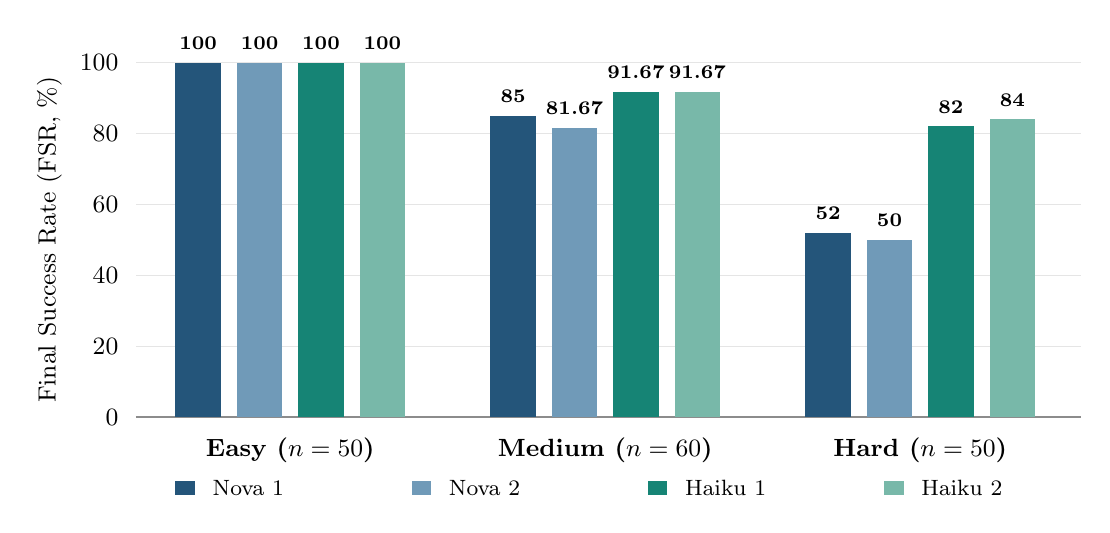
\begin{tikzpicture}[x=1cm,y=.045cm,font=\small]
\foreach \y in {0,20,40,60,80,100} {
  \draw[black!10] (0,\y) -- (12,\y);
  \node[anchor=east] at (-.1,\y) {\y};
}
\draw[black!45,line width=.6pt] (0,0) -- (12,0);
\node[rotate=90] at (-1.1,50) {Final Success Rate (FSR, \%)};
\fill[novaone] (0.5,0) rectangle (1.08,100);
\node[above,font=\scriptsize\bfseries] at (0.79,101) {100};
\fill[novatwo] (1.28,0) rectangle (1.8599999999999999,100);
\node[above,font=\scriptsize\bfseries] at (1.57,101) {100};
\fill[haikuone] (2.06,0) rectangle (2.64,100);
\node[above,font=\scriptsize\bfseries] at (2.35,101) {100};
\fill[haikutwo] (2.84,0) rectangle (3.42,100);
\node[above,font=\scriptsize\bfseries] at (3.13,101) {100};
\node[below,font=\small\bfseries] at (1.96,-3) {Easy ($n=50$)};
\fill[novaone] (4.5,0) rectangle (5.08,85);
\node[above,font=\scriptsize\bfseries] at (4.79,86) {85};
\fill[novatwo] (5.28,0) rectangle (5.86,81.66666666666666666666666667);
\node[above,font=\scriptsize\bfseries] at (5.57,82.66666666666666666666666667) {81.67};
\fill[haikuone] (6.0600000000000005,0) rectangle (6.640000000000001,91.66666666666666666666666667);
\node[above,font=\scriptsize\bfseries] at (6.3500000000000005,92.66666666666666666666666667) {91.67};
\fill[haikutwo] (6.84,0) rectangle (7.42,91.66666666666666666666666667);
\node[above,font=\scriptsize\bfseries] at (7.13,92.66666666666666666666666667) {91.67};
\node[below,font=\small\bfseries] at (5.96,-3) {Medium ($n=60$)};
\fill[novaone] (8.5,0) rectangle (9.08,52);
\node[above,font=\scriptsize\bfseries] at (8.79,53) {52};
\fill[novatwo] (9.28,0) rectangle (9.86,50);
\node[above,font=\scriptsize\bfseries] at (9.569999999999999,51) {50};
\fill[haikuone] (10.06,0) rectangle (10.64,82);
\node[above,font=\scriptsize\bfseries] at (10.35,83) {82};
\fill[haikutwo] (10.84,0) rectangle (11.42,84);
\node[above,font=\scriptsize\bfseries] at (11.129999999999999,85) {84};
\node[below,font=\small\bfseries] at (9.96,-3) {Hard ($n=50$)};
\fill[novaone] (0.5,-22) rectangle (0.75,-18);
\node[anchor=west,font=\footnotesize] at (0.85,-20) {Nova 1};
\fill[novatwo] (3.5,-22) rectangle (3.75,-18);
\node[anchor=west,font=\footnotesize] at (3.85,-20) {Nova 2};
\fill[haikuone] (6.5,-22) rectangle (6.75,-18);
\node[anchor=west,font=\footnotesize] at (6.85,-20) {Haiku 1};
\fill[haikutwo] (9.5,-22) rectangle (9.75,-18);
\node[anchor=west,font=\footnotesize] at (9.85,-20) {Haiku 2};
\end{tikzpicture}
\endgroup

\caption{Final Success Rate by difficulty, with percentages above the bars (Source: Author, 2026).}
\label{fig:results-difficulty}
\end{figure}

\subsubsection{Direct success and recovery within each group}
\hyperref[tab:results-difficulty-counts]{Table~\ref*{tab:results-difficulty-counts}}
compares final and clean direct successes within each difficulty group.
In Nova's first run, 23 of the 50 hard questions succeeded directly and three more
succeeded after recovery. This gave a CDSR of 46\% and an FSR of 52\%. 
The FDG was 6 percentage points.

\begin{table}[H]
\centering
{\small
\setlength{\tabcolsep}{4pt}
\begin{tabularx}{\textwidth}{@{}>{\raggedright\arraybackslash}Xrrrr@{}}
\toprule
\textbf{Group and measure} & \textbf{Nova 1} & \textbf{Nova 2} & \textbf{Haiku 1} & \textbf{Haiku 2} \\
\midrule
Easy: final / clean direct & 50 / 50 & 50 / 50 & 50 / 49 & 50 / 49 \\
\addlinespace[0.4em]
Medium: final / clean direct & 51 / 49 & 49 / 48 & 55 / 55 & 55 / 55 \\
\addlinespace[0.4em]
Hard: final / clean direct & 26 / 23 & 25 / 21 & 41 / 37 & 42 / 38 \\
\bottomrule
\end{tabularx}
}
\caption{Final and clean direct success counts by difficulty (Source: Author, 2026).}
\label{tab:results-difficulty-counts}
\end{table}

\hyperref[tab:results-difficulty-counts]{Table~\ref*{tab:results-difficulty-counts}}
shows that even though the models achieved perfect final accuracy on the easy group, 
it does not mean that their trajectories were identical.
Nova solved all 50 questions directly and on the first attempt. 
Haiku solved 49 directly and recovered on CB200-E030 in each run, 
giving a CDSR of 98\% and an FDG of 2 percentage points. 
On medium questions, all 55 of Haiku's successes were clean and direct. 
Nova, in contrast, recovered on two questions in run 1 and one in run 2. 
These counts explain why the same overall recovery
count was distributed differently across difficulty groups.

All remaining recoveries occurred on hard questions: three and four for
Nova, and four in each Haiku run. 
This resulted in Haiku's hard-question CDSR of 74\% and
76\%, compared with Nova's 46\% and 42\%. 
As a result, its advantage on this group remained when considering only clean direct successes.

The terminal failures also differed. In the hard group, Nova 1 had
18 semantic failures, five execution failures and one no-SQL outcome.
Nova 2 had 17 semantic failures and eight execution failures.
Haiku's nine and eight hard-question failures were all semantic failures
under the comparison contract. On medium questions, Nova 1's nine failures
were semantic; Nova 2 also had nine semantic failures and two execution failures.
Haiku had five semantic failures in each run.

\subsubsection{Long sequences within the difficulty groups}
The median SQL-attempt count was one in every group and run.
Nevertheless, \hyperref[tab:results-difficulty-attempts]{Table~\ref*{tab:results-difficulty-attempts}}
shows that this common median masked different distributions.
\hyperref[tab:results-difficulty-attempts]{The table} 
counts questions with more than two SQL attempts and gives
the longest sequence in each group. 
All remaining questions had at most two attempts, 
including the one no-SQL case already discussed.

\begin{table}[H]
\centering
{\small
\setlength{\tabcolsep}{4pt}
\begin{tabularx}{\textwidth}{@{}>{\raggedright\arraybackslash}Xrrrr@{}}
\toprule
\textbf{Group and measure} & \textbf{Nova 1} & \textbf{Nova 2} & \textbf{Haiku 1} & \textbf{Haiku 2} \\
\midrule
Easy: questions with $>2$ attempts & 0 & 0 & 0 & 0 \\
Easy: maximum attempts & 1 & 1 & 2 & 2 \\
\addlinespace[0.5em]
Medium: questions with $>2$ attempts & 1 & 2 & 0 & 0 \\
Medium: maximum attempts & 5 & 28 & 1 & 1 \\
\addlinespace[0.5em]
Hard: questions with $>2$ attempts & 5 & 10 & 0 & 0 \\
Hard: maximum attempts & 32 & 29 & 2 & 2 \\
\bottomrule
\end{tabularx}
}
\caption{Long SQL-attempt sequences by difficulty (Source: Author, 2026).}
\label{tab:results-difficulty-attempts}
\end{table}

More than two attempts occurred on 10\% of Nova's hard questions in run 1
and 20\% in run 2.
The medium-group proportions were 1.67\% and 3.33\%. 
Haiku had no such sequences in any difficulty group.

Long sequences were nevertheless not limited to hard questions.
In Nova's second run, the medium questions CB200-M039 and CB200-M051
used 28 and 24 attempts and both ended as execution failures.
Those two questions accounted for 52 of the medium group's 111 attempts
(46.85\%).
The other 58 questions used the remaining 59 attempts.
This shows that despite a median of one attempt, 
a few questions took up almost half the group's SQL activity.

For RQ4, harder questions coincided with lower FSR and CDSR for both models.
Harder questions also coincided with more long attempt sequences,
especially in Nova's hard group. 
These results show where the differences occurred, but the
individual trajectories are needed to explain what went wrong.